\documentclass[prb,twocolumn]{revtex4}
\usepackage{times}
\usepackage{bbm}
\usepackage[dvips]{graphicx}
\usepackage{latexsym,amsmath,amssymb,bm,euscript}
\usepackage[dvips]{color}
\usepackage{multirow}

\def\ra{\rangle} % bra
\def\la{\langle} % ket

\begin{document}

\title{}
\date{\today}
\pacs{}

\author{Scott D. Geraedts}
\author{Olexei I. Motrunich}
\affiliation{Department of Physics, California Institute of Technology, Pasadena, California 91125, USA}

%%%%%%%%%%%%%%%%%%%%%%%%%%%%%%%%%%%%%%%%%%%%%%%%%%%%%%%%%%%%%%%
\begin{abstract}
\end{abstract}
%%%%%%%%%%%%%%%%%%%%%%%%%%%%%%%%%%%%%%%%%%%%%%%%%%%%%%%%%%%%%%%
\maketitle

\section{$SO(3)$ spins as a Heisenberg model}
\label{section::Heisenberg}

\subsection{Bulk properties}
We will be studying the following action, in (3+1)-D Euclidean space-time:
\begin{equation}
S=S_{\rm spin}+\sum_{r,\mu} \frac{\lambda}{2}[ J_\mu(r)-c Q_\mu(r)]^2.
\label{action}
\end{equation}
$S_{\rm spin}$ is an action which penalizes fluctuations in the $SO(3)$ spins. The second term describes the binding between bosons and monopoles. The bosons, $J_\mu$, are represented by integer-valued conserved currents living on the links of a four-dimensional cubic lattice, where $r$ is the position on the lattice and $\mu$ is a direction. The $Q_\mu$ variables represent the monopoles, which are also integer-valued conserved currents. The parameter $c$ is an integer. When the real number $\lambda$ is large, this term will attach $c$ bosons to each monopole. We will work with periodic boundary conditions, in the case with no net charge and no net monopole number, so that the $J_\mu$ and $Q_\mu$ currents have winding number zero.


We will first represent the $SO(3)$ spins as unit vectors. This can be achieved with the following action, which describes a Heisenberg model:
\begin{equation}
S_{\rm spin}=\beta\sum_{R,\mu} \vec{n}(R)\cdot \vec{n}(R+\mu).
\end{equation}
Here $\vec{n}$ are unit vectors which represent the spins. They exist on a different lattice from the $J_\mu$ and $Q_\mu$ variables above. This lattice has its sites labelled by $R$, and they are at the centers of the (hyper)cubes of the lattice in Eq.~(\ref{action}). From these unit vectors, we can define the monopole current $Q_\mu$ using the prescription in Ref.~\onlinecite{LesikAshvin1}.
%more details about this?
 
\begin{itemize}
\item Explain how hedgehogs are constructed from spins
\item Monte Carlo details
\item How to measure current-current correlators, heat capacity, magnetization
\item Describe phase diagram, connect to model of uncoupled currents and spins
\item Discuss symmetries of model
\item Give easy-plane picture with 2 species of vortices sourced by monopoles
\item Show how Zeeman field in bulk breaks the phase
\item Show how c=2 is equivalent to c=0
\end{itemize}

\begin{figure}
\includegraphics[angle=-90,width=0.9\linewidth]{figures/bulklines.eps}
\caption{Inset: Phase diagram for the bulk of the Heisenberg version of the model. The phase diagram is equivalent to a system of decoupled currents and spins. At $\lambda=0$, the system has a paramagnet-ferromagnet transition as $\beta$ is increased. As $\lambda$ is increased, the boson currents bind to the monopole currents. The loops in the phases show a `snapshot' of the phase. Red loops mean that boson currents are proliferated in the phase, while blue loops indicate proliferated monopole currents. The phase of interest is the upper left is the `binding' phase where bosons are bound to monopoles. The main figure shows the current-current correlations of the bosons and monopoles as $\lambda$ is increased while $\beta=0$. We see that the correlators become equal as the system enters the upper left phase, indicating that bosons have bound to monopoles.}
\label{bulkphase1}
\end{figure}


\begin{figure}
\includegraphics[angle=-90,width=0.5\linewidth]{figures/monopoles.eps}
\caption{As discussed in the text, our system as two species of vortex lines (shown here as dotten and dashed). A monopole is a transition point between the two types of lines, with the charge of the monopole determined by the orientation of the vortex lines and their vorticity. Applying a Zeeman field to the surface means allowing only one type of vortex line through the surface. This leads to a correlation between the monopole charge and the vorticity at the surface, which is the origin of the Hall conductivity.}
\label{monopole}
\end{figure}

\subsection{Surface Properties}
%give surface details
\begin{itemize}
\item Show how surface is introduced
\item Discuss how measurements change when there is a surface
\item Explain how surface suppresses hedgehogs
\item Describe phase diagram, explain why none of the observed phases are evidence for topological behavior
\item Show how Zeeman field is introduced
\item Discuss how vortex-charge correlator measured
\item Explain hall conductivity in terms of easy-plane picture on slab
\item Discuss why the conductivity is quantitatively wrong
\end{itemize}

\begin{figure}
\includegraphics[angle=-90,width=0.9\linewidth]{figures/heissurf.eps}
\caption{The inset shows the phase diagram of the surface of the Heisenberg version of the model, without a Zeeman field. It was obtained by tuning the bulk into the phase where bosons and monopoles are bound, and then tuning $\beta$ and $\lambda$ {\em only on the surface}. If we have a topological phase, then the surface can either break a symmetry, have topological order, or gapless edge modes. We find that our surface always spontaneously breaks  a symmetry: either the bosons condense into a superfluid, or the spins align into a ferromagnet. This is consistent with the bulk being topological, but is also consistent with the bulk being topologically trivial. The main plot shows magnetization and boson current-current correlators, on a sweep in $\lambda_{\rm surf}$ for $\beta_{\rm surf}=0$. The magnetization is rescaled so that it is constant in system size in the disordered phase, and grows with system size in the ordered phase. The current-current correlators start to increase when the bosons condense. We see that there is no region where both the spins are disordered and the bosons gapped.}
\label{surfphase1}
\end{figure}

\begin{figure}
\includegraphics[angle=-90,width=0.9\linewidth]{figures/heishall.eps}
\caption{Hall conductivity for the Heisenberg version of the model. The $x$-axis is the strength of the Zeeman field. We see that as soon as a Zeeman field is turned on, the Hall conductivity takes a non-zero value. It was observed that all the observed conductivity comes from near the surfaces of the binding phase, and is evenly split between the top and bottom surfaces. However, the value is non-universal, due to lattice effects described in the main text. This prevents us from claiming that the Hall conducitivity must be due to the presence of a topological phase.}
\label{heishall}
\end{figure}

\section{$SO(3)$ spins using $CP^1$ representation}
\label{section::CP1}

\subsection{Bulk Properties}
The following action represents the $SO(3)$ spins in the $CP^1$ representation:
\begin{eqnarray}
&&S_{\rm spin}=-\beta\sum_{s=1,2}\sum_{\mu,R} (z_s^\dagger(R)z_s(R+\hat\mu)e^{-ia_\mu(R)}+c.c.) \nonumber\\
&&+\sum_{R,\mu<\nu} \cos[\nabla_\mu a_\nu(R)-\nabla_\nu a_\mu(R)].
\end{eqnarray} 
In this representation the $SO(3)$ spins are represented by two complex bosonic fields $z_1$,$z_2$. The spin, $\vec{n}$, can be extracted from the $z$ fields by writing them as a spinor $\mathbf{z}\equiv(z_1~z_2)^T$ and $\vec{n}=\mathbf{z^\dagger} \vec\sigma \mathbf{z}$, where the $\vec{\sigma}$ are Pauli matrices. The bosonic fields are minimally coupled to a compact gauge field $\vec{a}$. $F_{\mu\nu}\equiv \partial_\mu a_\nu-\partial_\nu a_\mu$, so the last term is similar to a Maxwell term for the compact gauge field. The variables in the above action live on a cubic lattice, where position on the lattice is given by $R$ and $\mu$,$\nu$ are directions.

We find it convenient to break the $SO(3)$ symmetry down to $U(1)\times\mathbb{Z}_2$ explicitly by taking the ``easy-plane'' limit of the $CP^1$ model. This means that we align all the spins $\vec{n}$ in the $xy$-plane. This corresponds to fixing the magnitude of $z_1$ and $z_2$, and allowing only phase fluctuations. The $CP^1$ model in the easy-plane limit becomes:
\begin{eqnarray}
&&S_{\rm spin}=-\beta\sum_{s=1,2}\sum_{\mu,R} \cos[\nabla_\mu\phi_s(R)-a_\mu(R)]\nonumber\\
&&+\sum_{R,\mu<\nu}\frac{K}{2}\left[\nabla_\mu a_\nu(R)-\nabla_\nu a_\mu(R)-2\pi B_{\mu\nu}(R)\right]^2.
\label{sspin}
\end{eqnarray}
Here $\phi_1$ and $\phi_2$ are $2\pi$-periodic variables which represent the phases of the boson fields. We have also rewritten the last term in a ``Villain'' form where the cosine is replaced by the above term, with $B_{\mu\nu}$ an unconstrained, integer-valued dynamical variable. The third term is therefore still a $2\pi$ periodic function of $F_{\mu\nu}$, and therefore this does not change the universality class of the problem.

Using the Villain form in the third term is advantageous as it allows us to define the monopole current:
\begin{equation}
Q_\mu(r)=\frac{1}{2}\epsilon_{\mu\nu\rho\sigma}\partial_\nu B_{\rho\sigma}(R).
\end{equation}
Note that $Q_\mu$ exists on the lattice labelled by $r$, while $B_{\mu\nu}$ is on the lattice labelled by $R$.

\begin{figure}
\includegraphics[angle=-90,width=0.9\linewidth]{figures/cp1bulkphase.eps}
\caption{Bulk phase diagram for the $CP^1$ version of the model. In addition to $\beta$ and $K$ axes in the figure, there is a third axis, $\lambda$, which is the strenght of the binding between bosons and monopoles. The locations of the phase transitions in the figure do not change $\lambda$ is increased, though at a critical value of $\lambda$ there is a phase transition to a phase where the bosons and monopoles are bound. The candidate for a topological phase is the Trivial Insulator at large $\lambda$.}
\label{cp1bulkphase}
\end{figure}

\begin{itemize}
\item Monte Carlo composite updates in this model
\item Discuss symmetries in easy-plane CP1
\item Show how magnetization is measured
\item Describe bulk phase diagram
\end{itemize}
\subsection{Surface properties}

\begin{itemize}
\item Describe surface phase diagram, how it is hedgehog-suppressed model, show how to measure photon-photom correlator
\item Show how Zeeman field is introduced
\item hall conductivity measurements, explain why we have gotten around the problems from the Heisenberg model
\item Mention that c=2 conductivity is trivial (show a plot?)
\end{itemize}

\begin{figure}
\includegraphics[angle=-90,width=0.9\linewidth]{figures/cp1surfphase.eps}
\caption{Surface phase diagram for the $CP^1$ version of the model. This diagram was obtained for $\beta_{\rm bulk}=0.2$, $K_{\rm bulk}=0.2$, $\lambda=8$, and parameters varied on the surface. The phase diagram has the same structure as the one found in the $NCCP^1$ model in Ref.~\cite{LesikAshvin2}. }
\label{cp1surfphase}
\end{figure}

\begin{figure}
\includegraphics[angle=-90,width=0.9\linewidth]{figures/cp1hall.eps}
\caption{Hall conductivity on the surface of the $CP^1$ version of the model. On each surface we find that the conductivity is quantized to $1/2$. This is half of the value allowed in a purely two-dimensional system. Since this value cannot be observed in a two-dimensional phase, the bulk of the system must be in a topological phase.}
\label{cp1hall}
\end{figure}

\section{Discussion}
%discussion of charges bound to monopoles (connections with Matthew)
\end{document}
